\documentclass[10pt,a4paper]{article}

\usepackage[utf8]{inputenc}
\usepackage[T1]{fontenc}
\usepackage{mathptmx}
\usepackage[margin=1.25cm,top=1.1cm,bottom=1.15cm]{geometry}
\usepackage{xcolor}
\usepackage{graphicx}
\usepackage{hyperref}
\usepackage{enumitem}
\usepackage{titlesec}
\usepackage{array}

\definecolor{cvblue}{HTML}{0875D1}
\hypersetup{
  colorlinks=true,
  urlcolor=cvblue,
  linkcolor=cvblue
}

\pagestyle{empty}
\setlength{\parindent}{0pt}
\setlength{\parskip}{0pt}
\setlist[itemize]{leftmargin=1.15em,itemsep=1pt,topsep=1pt,parsep=0pt}
\setlist[itemize,2]{label={-},leftmargin=1.5em,itemsep=1pt,topsep=0.5pt}
\titleformat{\section}
  {\color{cvblue}\Large\bfseries}
  {}
  {0pt}
  {}
  [\color{cvblue}\titlerule]
\titlespacing*{\section}{0pt}{5pt}{3pt}

\newcommand{\cvright}[1]{\hfill{\normalfont #1}}
\newcommand{\cvrole}[3]{%
  \item \textbf{#1:} #2 \cvright{#3}
}
\newcommand{\cvproject}[3]{%
  \item \textbf{#1} #2 \cvright{#3}
}
\newcommand{\cvedu}[4]{%
  \item \textbf{#1:} #2 \cvright{#3}\\
  \textit{Focus: #4}
}

\begin{document}
\small

\begin{minipage}[t]{0.82\textwidth}
  \centering
  {\Huge\bfseries\color{cvblue} Zeyu Wang}\\[4pt]
  Berlin, Germany \quad | \quad +49 170 6991380 \quad | \quad \href{mailto:wzy07777@gmail.com}{wzy07777@gmail.com}\\
  Date of Birth: 30.06.2003 \quad | \quad JiangSu Province, China\\
  LinkedIn: \href{https://www.linkedin.com/in/wang-zeyu-72b214395}{wang-zeyu-72b214395}
\end{minipage}
\begin{minipage}[t]{0.17\textwidth}
  \raggedleft
  % Upload zeyu_photo.png to the same Overleaf project folder.
  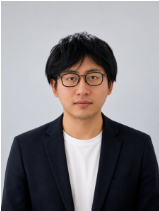
\includegraphics[width=1.9cm,height=2.55cm,keepaspectratio]{zeyu_photo.png}
\end{minipage}

\section*{Profile}
Computer Science M.Sc. student at TU Berlin and CKA/CKS-certified engineer targeting \textbf{Desktop Operations}, \textbf{IT Support} and \textbf{Junior System Administration} roles. Strong foundation in \textbf{Linux troubleshooting}, user-facing technical communication, Docker/Kubernetes environments, cloud deployments, health checks, backup and recovery runbooks, and automation with Go/Python scripts. German B2 and English C1 for daily support communication.

\section*{Skills}
\begin{itemize}
  \item \textbf{Desktop / IT Support:} issue triage, user support communication, software installation, environment setup, access and permission troubleshooting, technical documentation
  \item \textbf{Operating Systems:} \textbf{Linux administration}, shell/CLI tools, logs, services, file permissions; familiar with Windows/macOS desktop support basics
  \item \textbf{Networking / Services:} DNS, HTTP(S), reverse proxy basics, Caddy, health checks, REST/GraphQL APIs, SSH-based troubleshooting
  \item \textbf{Containers / Cloud:} \textbf{Docker}, Docker Compose, \textbf{Kubernetes}, Google Cloud Platform, AWS EC2/RDS, Cloudflare R2
  \item \textbf{Automation / Scripting:} Go, Python, Bash basics, Git, SQL migrations, backup and recovery scripts, operational runbooks
\end{itemize}

\section*{Certifications}
\begin{itemize}
  \item \textbf{CKA:} Certified Kubernetes Administrator \cvright{The Linux Foundation}
  \item \textbf{CKS:} Certified Kubernetes Security Specialist \cvright{The Linux Foundation}
\end{itemize}

\section*{Work Experience}
\begin{itemize}
  \cvrole{03.2024 - 06.2024}{Golang / Operations Engineer Intern, Part-time}{JH UniScheduler / Jhinno}
    \begin{itemize}
      \item Supported development and testing of a cloud resource management and job scheduling platform, with daily work around \textbf{Golang}, Linux command-line tooling and service troubleshooting.
      \item Worked with \textbf{Docker} and \textbf{Kubernetes} development environments, helping reproduce runtime issues, inspect logs and validate deployment behavior for containerized workloads.
      \item Assisted with operational documentation, environment setup notes and repeatable troubleshooting steps to improve handover between development and operations work.
      \item Also contributed to Jiaozi/Dumpling-related AI workflows, including RAG/fine-tuning data preparation and evaluation logs for a multi-agent AutoDL pipeline.
    \end{itemize}
\end{itemize}

\section*{Operations Projects}
\begin{itemize}
  \cvproject{03.2026 - Present:}{WeJoin - Cloud-Native Campus Platform}{\href{https://wejoin.store}{wejoin.store}}
    \begin{itemize}
      \item \textbf{Tech Stack:} Go/Gin, React, TypeScript, PostgreSQL/PostGIS, Redis, Cloudflare R2, Docker Compose, Caddy, Terraform, Ansible.
      \item Built and operated a Docker Compose deployment with Caddy reverse proxy, database services, object storage integration and environment-based configuration.
      \item Added \textbf{health checks}, tracked SQL migrations, backup and recovery runbooks, and deployment documentation for reliable day-to-day operations.
    \end{itemize}

  \cvproject{06.2026 - Present:}{MiSArch Agent Gateway - Service Integration on GCP}{Go, Docker, GCP}
    \begin{itemize}
      \item \textbf{Tech Stack:} Go, GraphQL, MCP, Docker Compose, Google Cloud Platform, Linux VM, Python smoke-test scripts.
      \item Deployed MiSArch microservices and a Go gateway on a \textbf{GCP Compute Engine} VM, including firewall-limited public access, health/readiness endpoints and Docker network configuration.
      \item Troubleshot service connectivity between external clients, the gateway container and the internal GraphQL endpoint; documented repeatable commands for logs, readiness checks and endpoint validation.
    \end{itemize}

  \item \textbf{Linux / Container Operations Practice}
    \begin{itemize}
      \item \textbf{Tech Stack:} Linux, Docker, Kubernetes, Bash/Python, Go, Git.
      \item Regularly used Linux shell tools, Git workflows, container builds, local service checks and scripted smoke tests to validate backend and cloud-native projects.
      \item Practiced incident-style debugging: checking configuration, reproducing failures, reading logs, validating network endpoints and writing concise recovery notes.
    \end{itemize}
\end{itemize}

\section*{Education}
\begin{itemize}
  \cvedu{10.2025 - 07.2027}{Computer Science, M.Sc.}{Technical University Berlin}{Cloud Infrastructure, Kubernetes, Docker, Ansible, AI Agent}
  \cvedu{09.2021 - 06.2025}{Computer Software Engineering, Bachelor}{Xidian University}{Computer Science, Software Engineering, Go Development}
\end{itemize}

\section*{Languages}
\begin{itemize}
  \item Chinese \cvright{Native}
  \item German \cvright{B2}
  \item English \cvright{C1}
\end{itemize}

\end{document}
